\begin{enumerate}[label=\thesection.\arabic*.,ref=\thesection.\theenumi]
\numberwithin{equation}{enumi}

\item
Write the general expression for the transfer function of a Phase lag-lead compensator. 
\solution
The Transfer Function of the Phase lag-lead compensator is
\begin{align}
\label{eq:ee18btech11044_hs_gen}
    H(s) = \frac{(1+ \alpha s T_1)(1+ \beta s T_2)}{(1+T_1 s)(1 + T_2 s)}
\end{align}
$\alpha$ and $\beta$ are generally chosen in such a way that
\begin{align}
    \alpha \beta = 1
\end{align}
%
\item Write the expression for phase introduced by phase lag-lead compensator. 
\solution 
\begin{multline}
    \phi = \tan^{-1}\brak{\frac{\omega T_1}{\beta}} + \tan^{-1}\brak{ \beta \omega T_2} 
\\
- \tan^{-1}\brak{\omega T_1} - \tan^{-1}\brak{\omega T_2}
\end{multline}

\item Consider the Transfer function of a phase lag-lead compensator
\begin{align}
    C(s) = \frac{(1+\frac{s}{0.1})(1+\frac{s}{100})}{(1+\frac{s}{1})(1+\frac{s}{10})}
\label{eq:ee18btech11044_hs_ex}
\end{align}
Find the frequency range in which the phase (lead) introduced by the compensator reaches the maximum 
\\
\solution From \eqref{eq:ee18btech11044_hs_gen} and \eqref{eq:ee18btech11044_hs_ex},
\begin{align}
\alpha &= 10, T_1 = 1,
\\
\beta &= 0.1, T_2 = 0.1.
\end{align}
%The phase of 
%Comparing the given Transfer function with with equation(1.7.1), we get 
%Substituting these values in equation (1.8.1)
Thus, 
\begin{multline}
   \angle C(\j\omega) = \underbrace{\tan^{-1}(10\omega) - \tan^{-1}(\omega)}_{lead} + 
\\
\underbrace{\tan^{-1}(0.01\omega)  - \tan^{-1}(0.1\omega)}_{lag}
\end{multline}
As we are trying to find the range of frequencies in which phase lead introduced by the compensator is maximum, the phase introduced by the lag part of compensator will be close to zero.  Hence, the problem can be expressed as
\begin{align}
\min_{\omega}     \tan^{-1}(10 \omega ) - \tan^{-1}(\omega )
\end{align}
which can be obtained by 
\begin{align}
\frac{d}{d\omega}\sbrak{\tan^{-1}(10 \omega ) - \tan^{-1}(\omega )} &= 0
\\
\implies \frac{10}{1+100\omega^2} - \frac{1}{1+\omega^2} &= 0
\\
\text{or, }  \omega &= \frac{1}{\sqrt{10}}
\end{align}
\item Verify your result using a python plot.
\\
\solution The following code
\begin{lstlisting}
codes/ee18btech11044.py
\end{lstlisting}
%
generates Fig. \ref{fig:ee18btech11044}.

\begin{figure}[!ht]
\centering
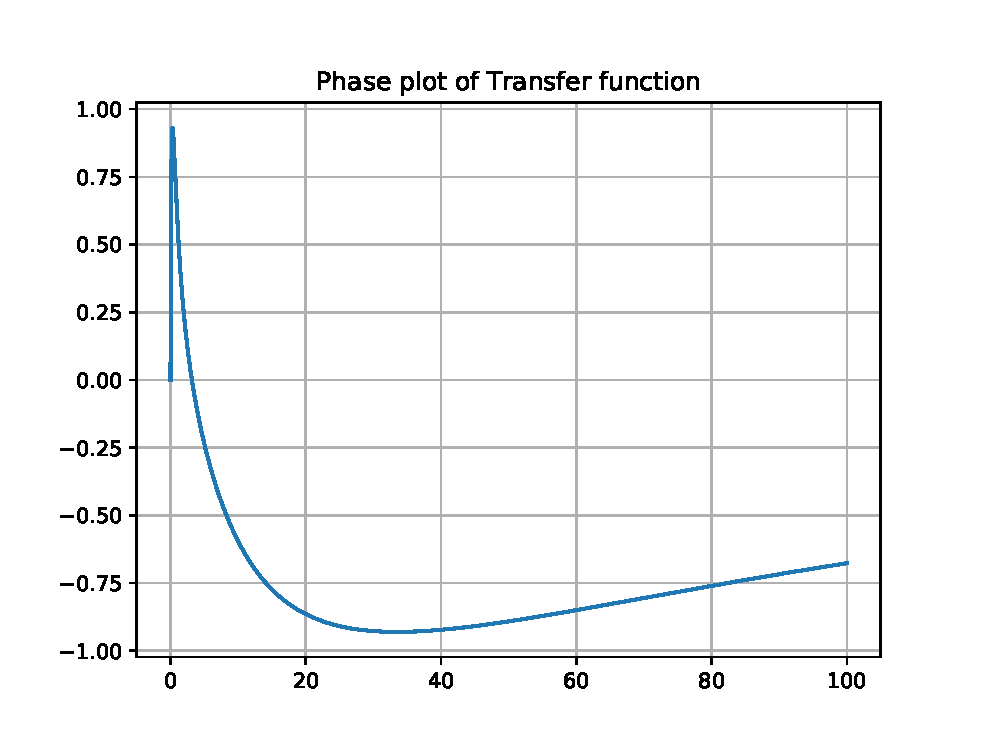
\includegraphics[width=\columnwidth]{./figs/EE18BTECH11044.eps}
\caption{}
\label{fig:ee18btech11044}
\end{figure}


\end{enumerate}
